\chapter{Architectural Design}
\labch{options}
	\section{Overview}
		From an implementation perspective, it was decided to develop the S\&C platform as a web application.For this reason, the architecture chosen for its development is a 3-tier architecture. It is a software design pattern that separates applications into three distinct layers:
		\begin{enumerate}
			\item \textbf{Presentation Layer}: The user interface (UI) where users interact with the application
			\item \textbf{Application Layer}: the layer in which the data are processed
			\item \textbf{Data Layer}: manages the storage, retrieval, and manipulation of data, involving databases
		\end{enumerate}
		
		This architecture offers significant advantages in terms of scalability, maintainability, and especially modularity, allowing each layer to be developed and updated independently of the others.
		
		Going into detail, the data layer employs two different types of databases: a relational database is used to manage the structured data of our system, which constitutes the majority of the data utilized by the platform (users, internship advice, internships, notifications, etc.). For the management of unstructured data, namely CVs and selection-related questionnaires, a non-relational database was chosen. Specifically, MongoDB was selected, as its JSON-based data storage format is perfectly suited for hierarchical and non-rigid structures, such as CVs and questionnaires.
		
		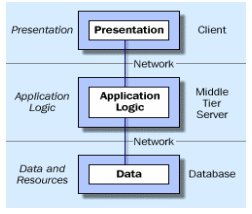
\includegraphics{3Tier.jpg}
		
		\section{Component View}
			As mentioned, the platform is developed used a 3-tier architecture approach with 2 DB(a RDBMS and MongoDB); As for the back-end components, four main macro-components can be identified, which are:
			\begin{enumerate}
				\item \textbf{Social Application System}: It provides the "social" functionalities of the platform, such as user registration/login, searching for internship advice, viewing profiles, applying for/sending an application proposal, sending feedback/complaints, and so on. It is divided in several components:
				\begin{enumerate}
					\item \textbf{Authentication Manager}: It handles user authentication (initial registration, subsequent logins);
					\item \textbf{Application Manager}: It is responsible for managing application proposals, acceptances, and application requests;
					\item \textbf{Advice Presenter}: It provides functionalities for viewing individual internship advice and the list of all internship advice published on the platform;
					\item \textbf{Advice Publisher}: It provides functionalities for publishing an internship advice;
					\item \textbf{Feedback Manager}: It provides functionalities for viewing feedback questionnaires and receiving the corresponding responses;
					\item \textbf{Internship Manager}: It displays the ongoing internships (both the list and individual ones) and manages user complaints;
					\item \textbf{Profile Manager}: it provides functionalities for managing a profile, from creation to modification and deletion
					\item \textbf{Profile Presenter}: It allows viewing profiles
					\end{enumerate}
					
					\item \textbf{Recommendation System}: It is the component responsible for the recommendation functionality offered by the platform, which involves analyzing the necessary information (feedback, CVs for students, etc.), determining which internships/students may be of interest to a specific user, and finally sending this information to the interested user. It is divided into 3 sub-components:
					\begin{enumerate}
						\item \textbf{Recommendation Interface}: It is the component that retrieves the necessary information from the databases to develop the recommendation;
						\item \textbf{Recommendation Analyzer}: t is the component that performs the analysis on the information obtained from the recommendation interface (feedback, CVs, etc.);
						\item \textbf{Recommendation Presenter}: It inserts the recommendation results into the database and triggers the sending of notifications to inform that the recommendation has been made
					\end{enumerate}
					
					\item \textbf{Selection Management System}: 
					It provides functionalities related to the entire selection process, from its configuration to the sending of results. It is divided in 3 sub-components:
					\begin{enumerate}
						\item \textbf{SP Initializer}: It provides functionalities for configuring the selection process (dates, metrics, questionnaires, etc.);
						\item \textbf{SP Manager}: It manages the insertion of answers in the questionnaires and the subsequent finalization of the selection process
						\item \textbf{SP presenter}: It displays interview dates and the results of the selection process
					\end{enumerate}
					
					\item \textbf{Notification System}: 
					It is the component responsible for managing all notifications generated and sent by the system; it handles the creation, sending, and triggering of notifications with the mail service. It is divided in 2 sub-components:
					\begin{enumerate}
						\item \textbf{Notification presenter}: It allows viewing notifications (both individual ones and the list);
						\item \textbf{Notification Generator}: It is the component that generates a notification and triggers the sending of an email;
					\end{enumerate}
			\end{enumerate}
			
			there are other important components of the system:
			\begin{enumerate}
				\item \textbf{DBMS}: stores all the structured data of the platform
				\item \textbf {WebServer}: it is the component related to routing the incoming request to the appropriate internal component.
				\item \textbf{MongoDB API}: A programming interface that allows developers to interact with a MongoDB database through HTTP requests, using CRUD operations (Create, Read, Update, Delete) on data stored in a MongoDB database;
				\item \textbf{SES API}: Amazon Simple Email Service (SES) is an email sending and receiving service offered by Amazon Web Services (AWS). The SES API allows to easily integrate email sending functionality into applications/websites.
			
			\end{enumerate}
			
			for the front-end, there are 2 clients which interact with the back-end:
			\begin{enumerate}
				\item \textbf{WebClient}: the UI of the application; it interacts with the back-end through REST API, which is based on a set of principles and constraints that allow systems to communicate over the web using standard HTTP methods such as GET, POST, PUT, DELETE, etc.
				\item \textbf{Client Mail}: the client used to access and manage the mail; it communicates with the back-end (in particular with the Notification system) through SES API
			\end{enumerate}
			
			the component diagram is shown in the following figure:
			
			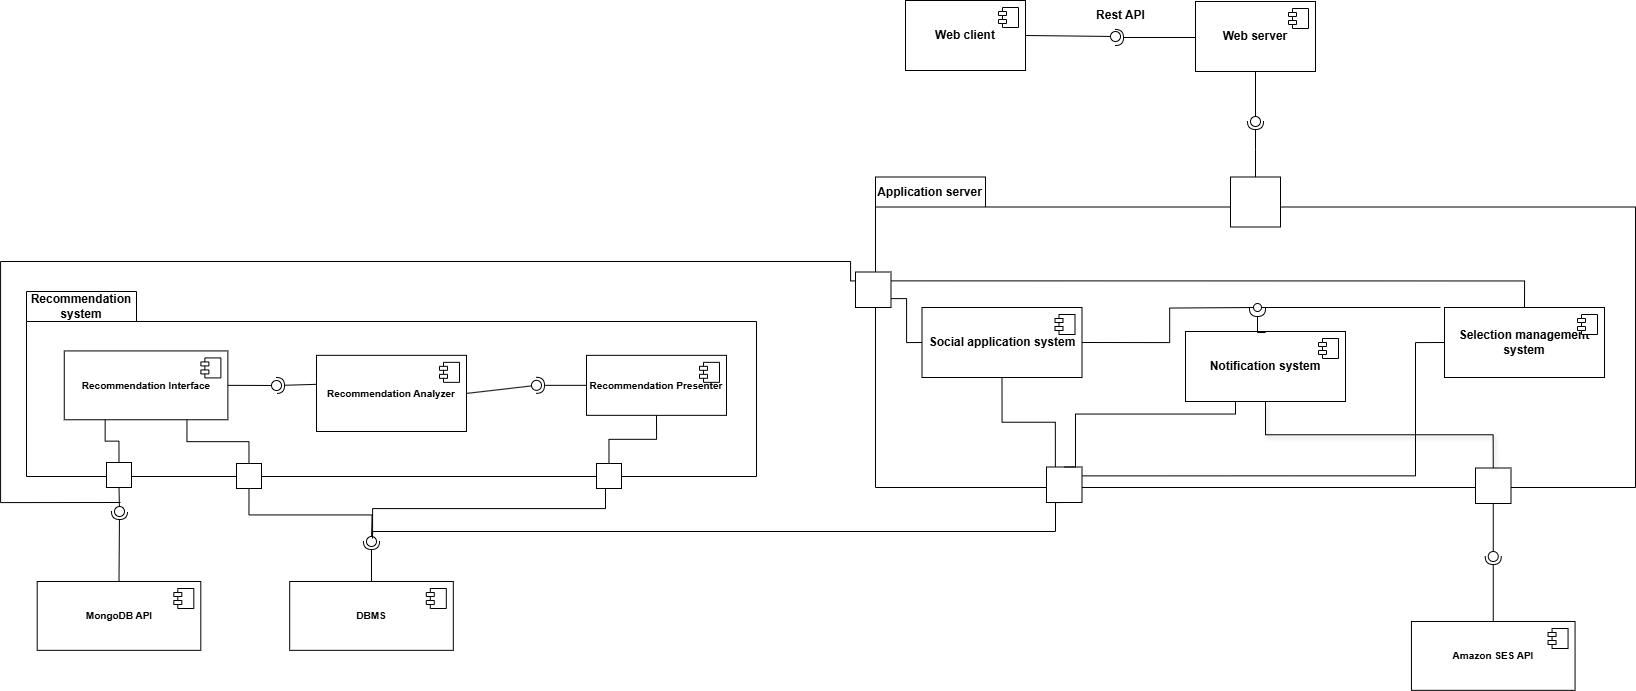
\includegraphics{componentView.png}
			
			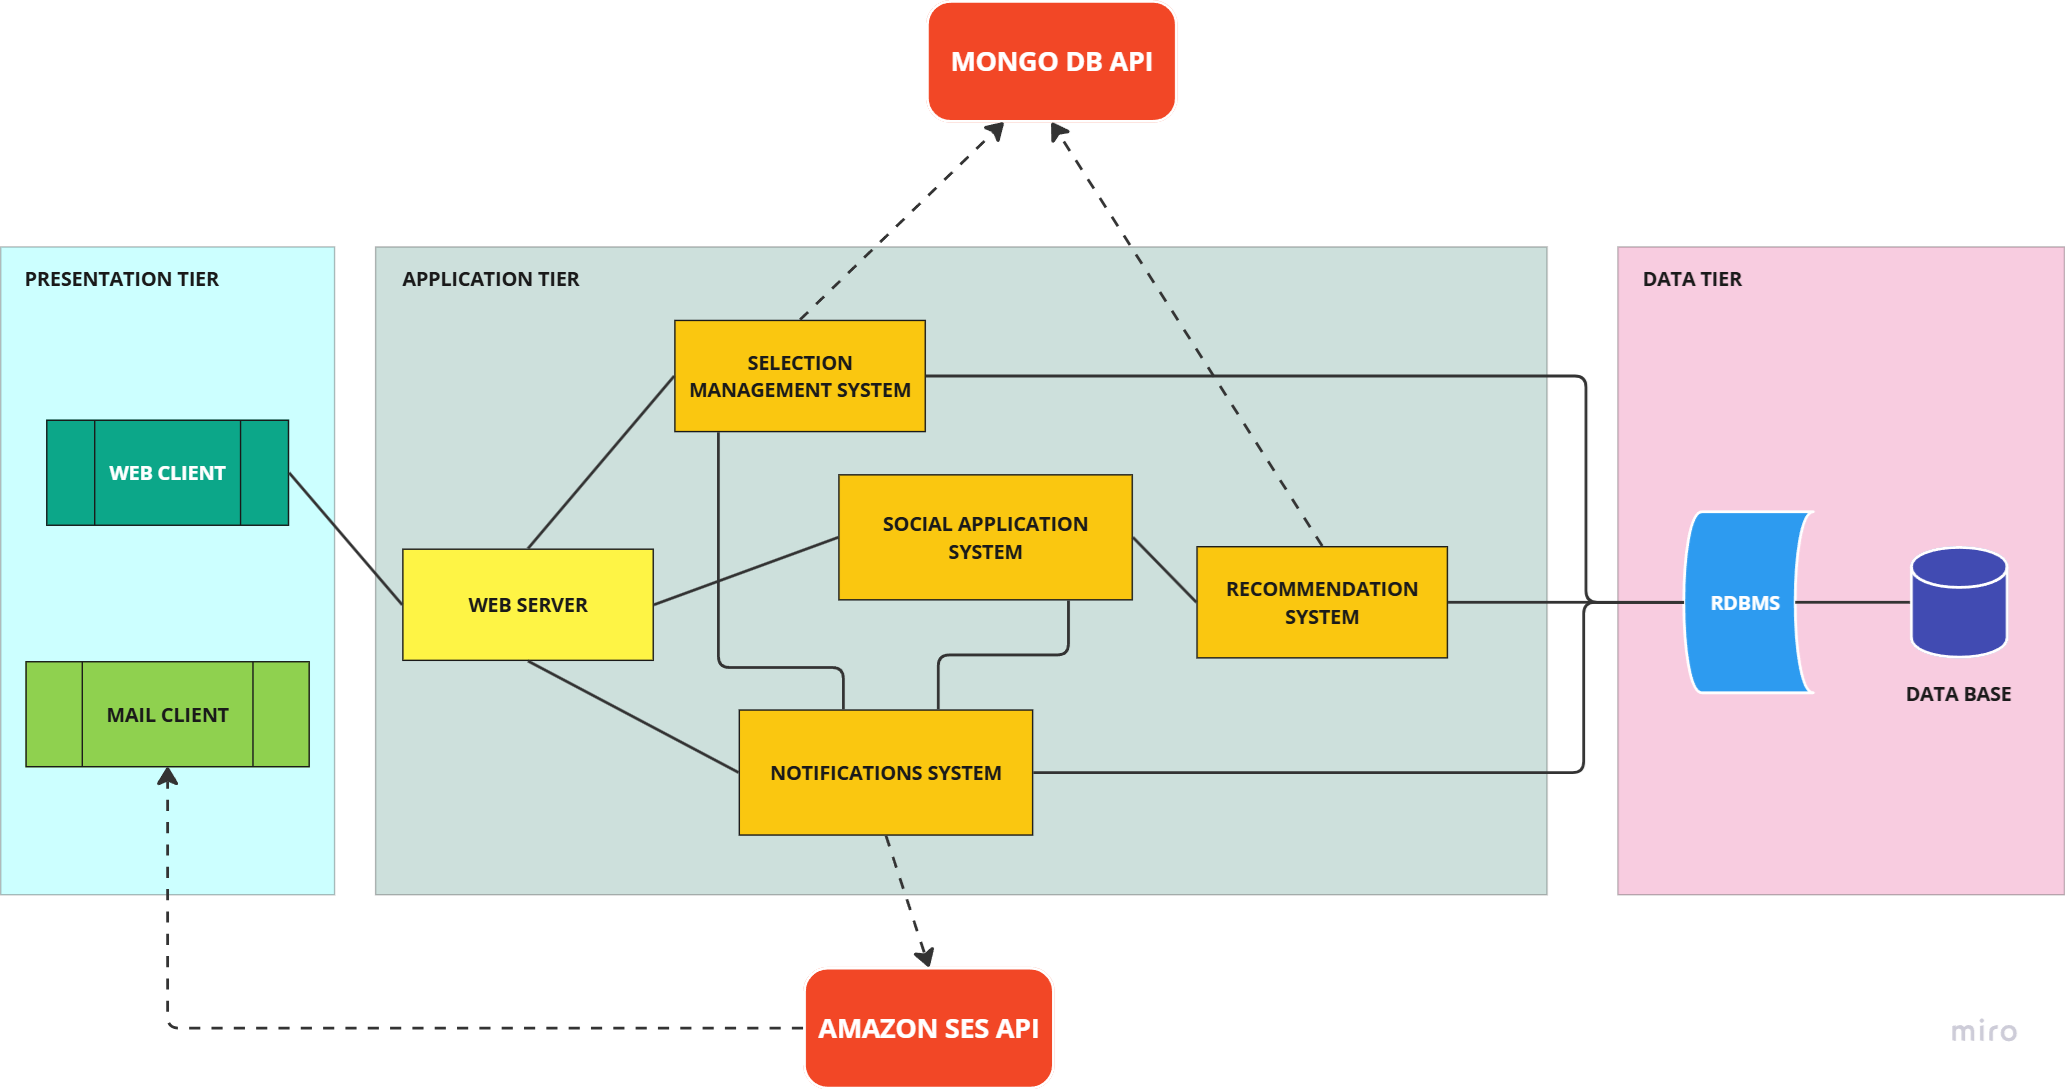
\includegraphics{informalArc.png}
	
	\section{Deployment View}
	\section{Runtime View}
		\begin{figure}[H]
			\centering
			{\bfseries [UC1] - Student Registration}
			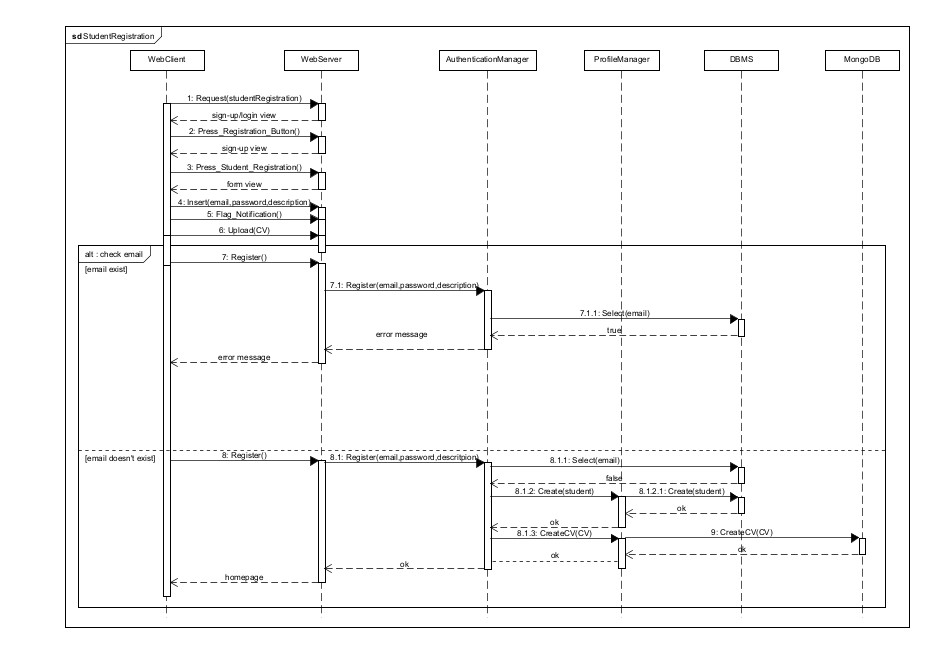
\includegraphics[scale=0.3]{StudentRegistrationDD.jpg}
			\caption{[UC1] - Student Registration}
		\end{figure}
			
		The figure shows the student registration process; the request is sent to Authentication Manager, which is also responsible for receiving the registration form completed by the student. Once received, Authentication Manager queries the DBMS to check if the student's email is already present in the database. If it is not present, the student will be saved in the database, while the CV will be stored in MongoDB as an unstructured data. If the email is already in the database, an error message will be displayed to the student.
		
		\begin{figure}[H]
			\centering
			{\bfseries [UC2] - Company Registration}
			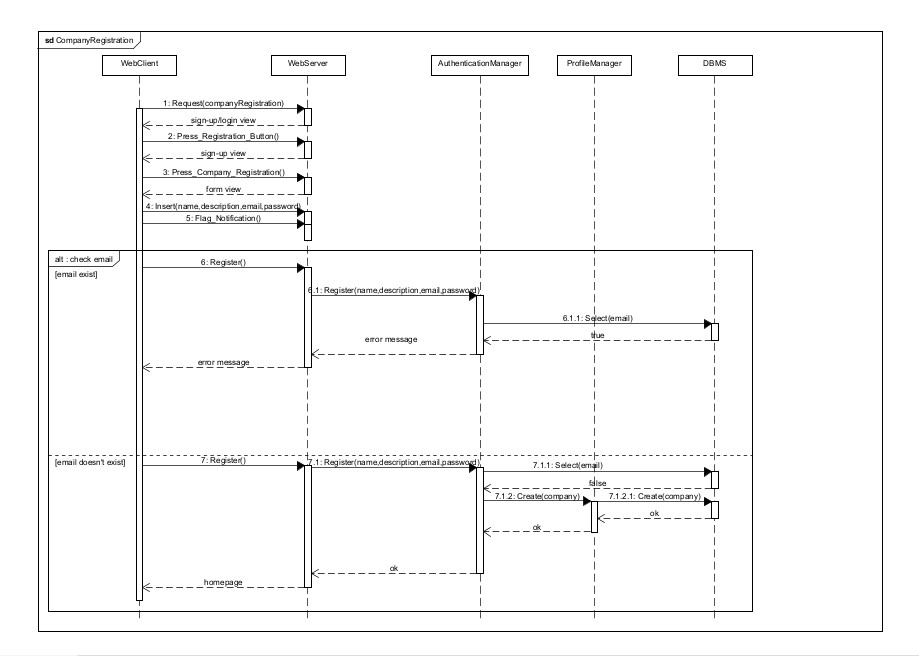
\includegraphics[scale=0.3]{CompanyRegistrationDD.jpg}
			\caption{[UC2] - Company Registration}
		\end{figure}
		
		The figure shows the company registration process; the flow is similar to the student registration case, with the difference that in this case, different data is saved (the company has a name and a description), and all the data is stored in the relational database since they are all structured data.
		
		\begin{figure}[H]
			\centering
			{\bfseries [UC3] - User Login}
			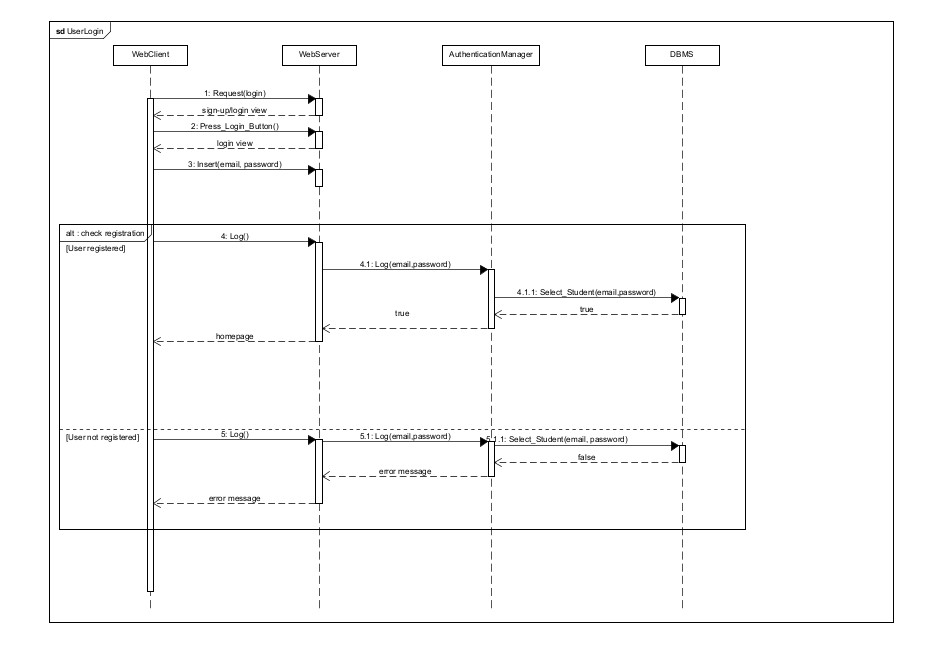
\includegraphics[scale=0.3]{UserLoginDD.jpg}
			\caption{[UC3] - User Login}
		\end{figure}
		
		The figure shows the user login process, which is similar for both students and companies; in this case, the request is handled by the Authentication Manager, which selects the student from the database to allow login. If the student is not found, an error message is displayed.
	\section{Component Interfaces}
	\section{Data Logic Model}
		Starting from the high-level class diagram presented in the RASD, the logic scheme of the database is designed:
		\begin{figure}[H]
			\centering
			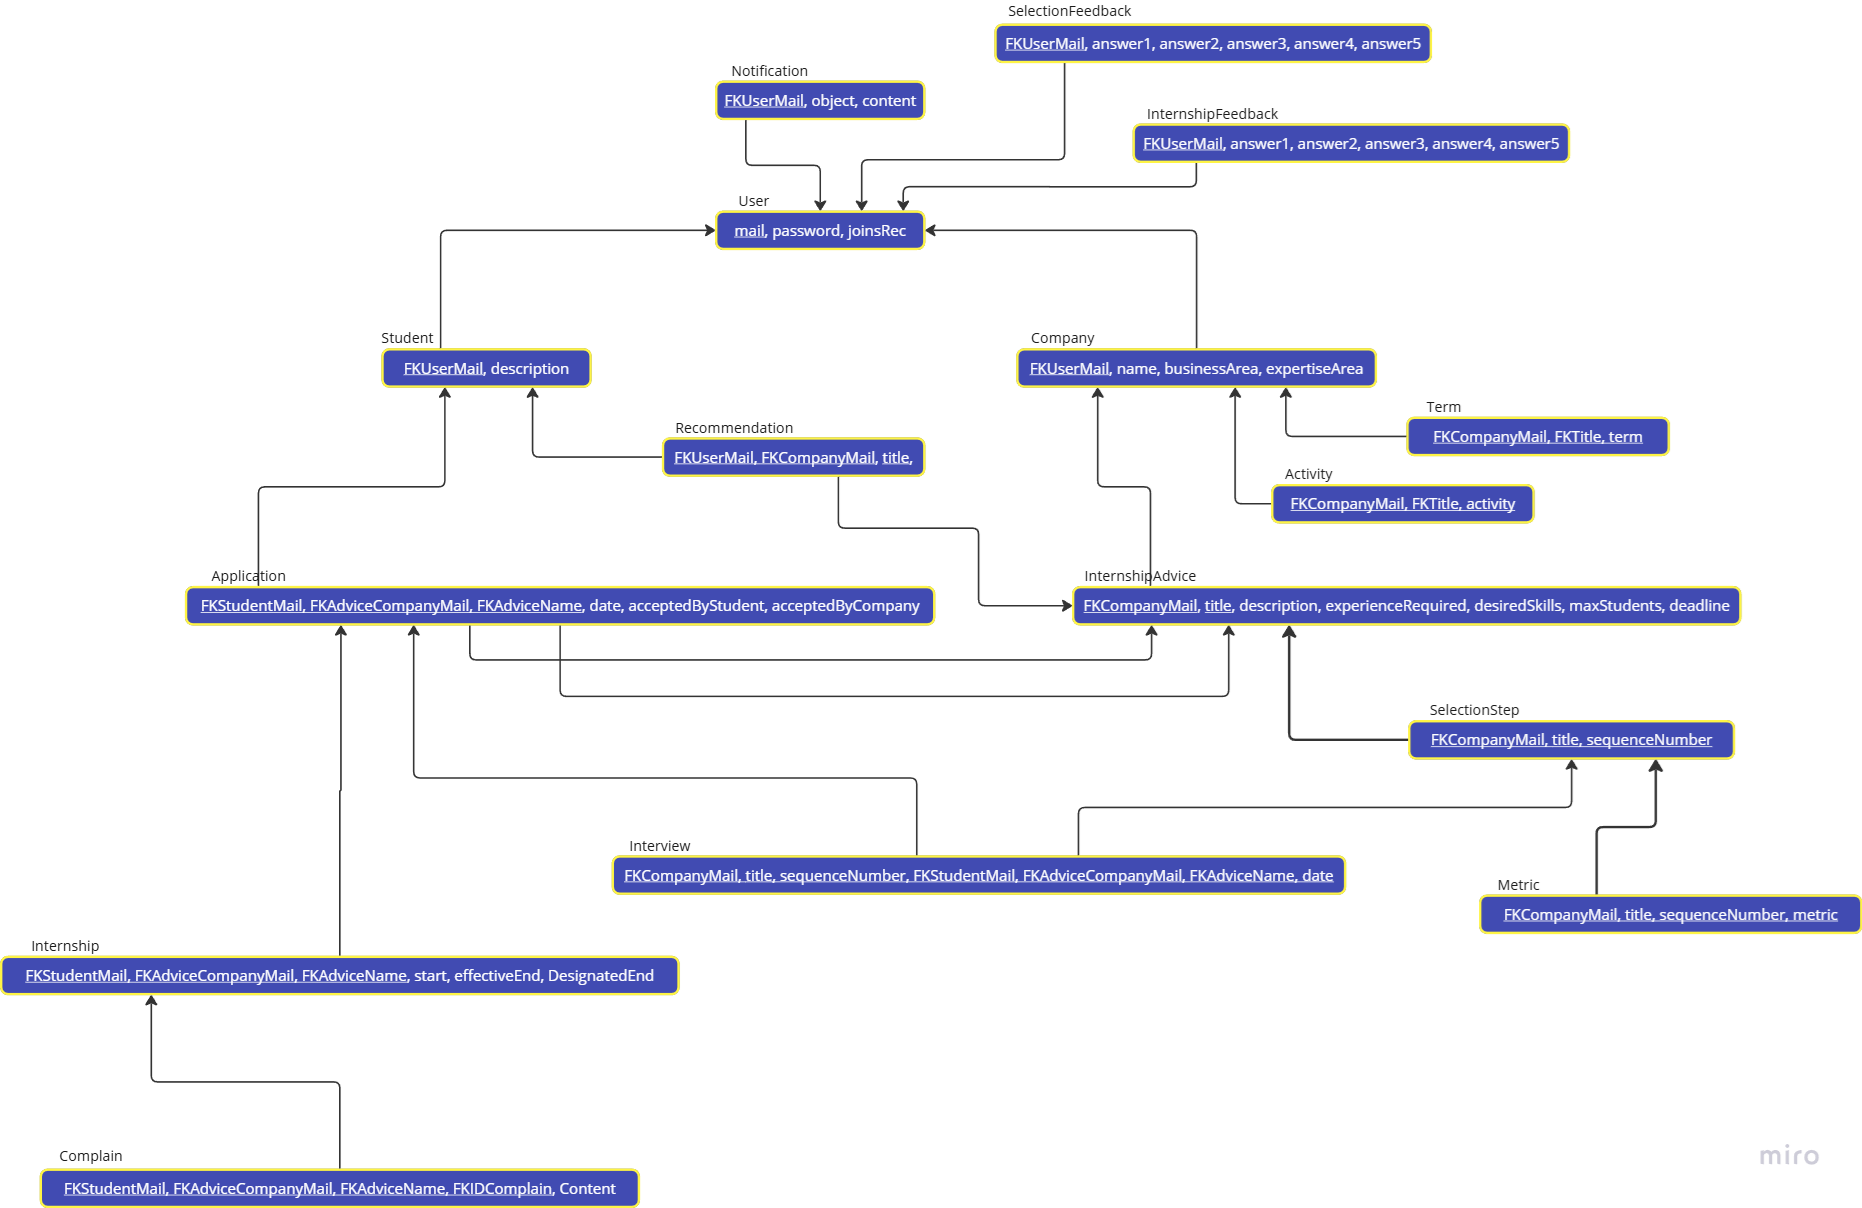
\includegraphics{datalogic.png}
			\caption{Data logic model scheme}
		\end{figure}
		Classes are almost one-to-one mapped with tables (with reification of vector attributes), the only relevant differences are:
		\begin{itemize}
			\item feedback-tables has an attribute for each questionnaire answer, this is not a concern since questionnaires are static (each questionnaire always has the same set of questions);
			\item the \emph{Recommendation} table was added, in order to store the recommendation analysis results;
			\item selection process questionnaires and CVs are missing since they are stored in Mongo DB (they are far more suitable for an unstructured data representation).
		\end{itemize}
	\section{Selected Architectural Styles and Patterns}